\documentclass[tikz,border=10pt]{standalone}
\usepackage{pgfplots}
\pgfplotsset{compat=1.18}
\usepackage{amsmath,amssymb,bm}
\definecolor{darkbg}{HTML}{ffffff}
\definecolor{lightfg}{HTML}{333333}
\definecolor{accent}{HTML}{2d7d46}
\definecolor{accent2}{HTML}{2d6d7d}
\definecolor{mutedcol}{HTML}{888888}
\definecolor{bordercol}{HTML}{cccccc}
\definecolor{redcol}{HTML}{cc3333}
\definecolor{bluecol}{HTML}{3355bb}
\color{lightfg}

\begin{document}
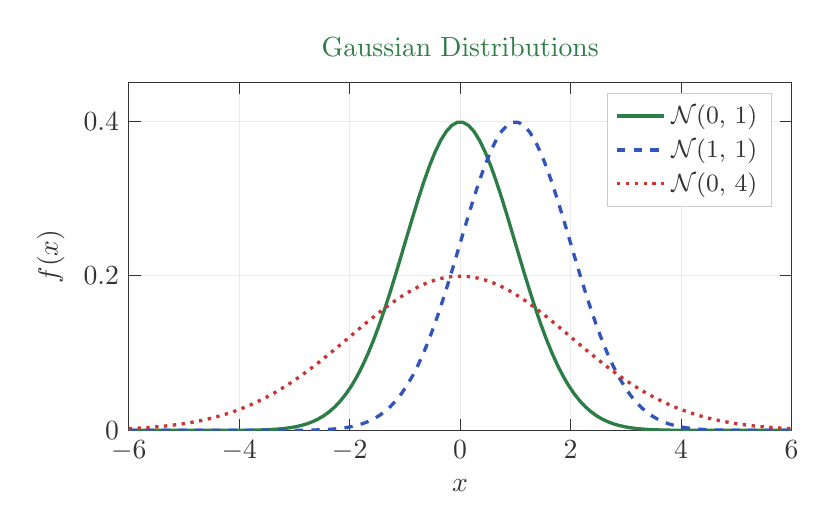
\begin{tikzpicture}
\begin{axis}[
  width=10cm, height=6cm,
  axis background/.style={fill=darkbg},
  axis line style={lightfg},
  tick style={lightfg},
  ticklabel style={color=lightfg},
  label style={color=lightfg},
  title style={color=accent},
  legend style={fill=darkbg, draw=bordercol, text=lightfg, font=\small},
  grid style={draw=bordercol, opacity=0.4},
  xlabel={$x$},
  ylabel={$f(x)$},
  title={Gaussian Distributions},
  domain=-6:6,
  samples=120,
  xmin=-6, xmax=6,
  ymin=0, ymax=0.45,
  grid=major,
  every axis plot/.style={very thick},
  legend pos=north east,
]

% N(0,1): mu=0, sigma=1
\addplot[accent, solid]
  {1/(1*sqrt(2*pi))*exp(-((x-0)^2)/(2*1^2))};
\addlegendentry{$\mathcal{N}(0,\,1)$}

% N(1,1): mu=1, sigma=1
\addplot[bluecol, dashed]
  {1/(1*sqrt(2*pi))*exp(-((x-1)^2)/(2*1^2))};
\addlegendentry{$\mathcal{N}(1,\,1)$}

% N(0,4): mu=0, sigma=2
\addplot[redcol, dotted]
  {1/(2*sqrt(2*pi))*exp(-((x-0)^2)/(2*2^2))};
\addlegendentry{$\mathcal{N}(0,\,4)$}

\end{axis}
\end{tikzpicture}
\end{document}
